\section{Zufallsvariablen}
%\listoftodos

\begin{bsp}
		$1$ mal würfeln. \\

		$\begin{aligned}
			 \underset{(Omega)}{\Omega} &= \text{ Menge der möglichen Ausgänge} \\
																	&= \text{ Ergebnisse } 
		\end{aligned}$

\hfill
		\begin{tikzpicture}[scale=0.7,baseline={(current bounding box.center)}]
		%	\draw[help lines] (0,0) grid (8,5);
			\draw (2,0) -- (2,5) -- (8,5) -- (8,0) -- (2,0);
			\node[rotate=0] at (3,4) {\LARGE 1};
			\node[rotate=10] at (4,3) {\LARGE 2};
			\node[rotate=-0] at (5,4) {\LARGE 3};
			\node[rotate=-0] at (6.1,2.3) {\LARGE 4};
			\node[rotate=-20] at (4.3,1.5) {\LARGE 5};
			\node[rotate=0] at (5.2,1) {\LARGE 6};
			\draw [->] (2,2.3) -- (0,2.3);
		\end{tikzpicture}
%
\vspace{-0.01\textheight}
	\begin{itemize}[]
		\item% 
			\begin{flalign*}
			P(A) & = P (\text{gerade Zahlen})  \\
					 & = P(\hspace{-1.0em} \underbrace{ \set{2,4,6} }
							_{\substack{\text{Anzahl der } \\ \text{günstigen Erg.}}} \hspace{-1.0em}) 
						 = \frac{\text{Anzahl der günstigen Ergebnisse}}
							{\underbrace{\text{Anzahl der möglichen Ergebnisse}}_
							{\substack{= \text{Anzahl d. Elemente in } \Omega}}} 
						 = \frac{3}{6}\\
					 &\\
			 P (\set{1}) &= \frac{1}{6}\\ 
			\end{flalign*}	
	\end{itemize}

\begin{minipage}{0.4\linewidth}
	\begin{tikzpicture}[scale=0.7]
		%\draw[help lines] (0,0) grid (8,5);
		% Box mit Omega
		\draw (2,0.5) -- (2,4.5) -- (7.5,4.5) -- (7.5,0.5) -- (2,0.5);
		\node at (1,4.5) {\Huge $\Omega$};
		% Zahlen in der Box
		\foreach \x/\y/\n/\r in {2.7/3.5/1/0,2.9/1.8/2/5,4.7/3.5/3/7,4.7/1.2/4/-5,6.7/3.5/5/0,6.9/1.5/6/0}
		\node[rotate=\r] at (\x,\y) {\LARGE \n};
		% Zahlen ausserhalb der Box
		\foreach \x/\y/\n/\r in {2.7/3.5/1/0,2.9/1.8/2/5,4.7/3.5/3/7,4.7/1.2/4/-5,6.7/3.5/5/0,6.9/1.5/6/0}
		\ifthenelse{\equal{\n}{1} \OR \equal{\n}{3} \OR \equal{\n}{5}}%
			{\node at (\x+0.4,\y+1.6) {\LARGE \n}}%
			{\node at (\x+0.1,-0.5) {\LARGE \n}};
		% Zeichnet die Pfeile
		\foreach \x/\y/\n/\r in {2.7/3.5/1/0,2.9/1.8/2/5,4.7/3.5/3/7,4.7/1.2/4/-5,6.7/3.5/5/0,6.9/1.5/6/0}
		\ifthenelse{\equal{\n}{1} \OR \equal{\n}{3} \OR \equal{\n}{5}}%
			{\draw[thick,->] (\x,\y+0.5) -- (\x+0.34,\y+1.2)}%
			{\draw[thick,->] (\x,\y-0.5) -- (\x+0.1,-0.1)};
	\end{tikzpicture}
\end{minipage}
%
\begin{minipage}{0.6\linewidth}
	ZV $X = $ Augenzahl\\
	Wahrscheinlichkeitsverteilung
	\def \var {0.10\linewidth}
	\begin{tabular}{m{0.28\linewidth}|m{\var} m{\var}m{\var}m{\var}m{\var}m{\var}}
		\centering $x_i$  & 1 & 2 & 3 & 4 & 5 & 6 \tabularnewline
		\hline
		\centering $P(X = x_i)$ & $\frac{1}{6}$ & $\frac{1}{6}$ & $\frac{1}{6}$
														& $\frac{1}{6}$ & $\frac{1}{6}$ & $\frac{1}{6}$
	\label{Wahrscheinlichkeitsverteilung}
	\end{tabular}
\end{minipage}
~\\
\begin{minipage}{0.45\linewidth}
	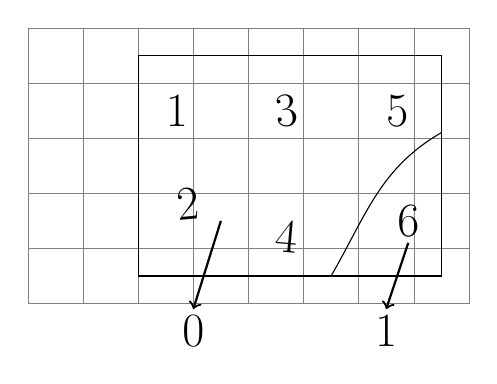
\begin{tikzpicture}[scale=0.7]
		\draw[help lines] (0,0) grid (8,5);
		% Box mit Omega
		\draw (2,0.5) -- (2,4.5) -- (7.5,4.5) -- (7.5,0.5) -- (2,0.5);
		% Zahlen in der Box
		\foreach \x/\y/\n/\r in {2.7/3.5/1/0,2.9/1.8/2/5,4.7/3.5/3/7,4.7/1.2/4/-5,6.7/3.5/5/0,6.9/1.5/6/0}
		\node[rotate=\r] at (\x,\y) {\LARGE \n};
		% Schrägstrich in der Box 
		\draw (5.5,0.5) to [out=60,in=-150] (7.5,3.1);
		% Pfeile an den Unterteilung : 0
			%definiere (lokale Variabeln)
			\def \x {3} 
			\def \y {-0.1}
		\draw[thick,->] (\x+0.5,1.5) -- (\x,\y);
		\node at (\x,\y-0.4) {\LARGE 0};
		% Pfeile an den Unterteilung : 1
			%definiere (lokale Variabeln)
			\def \x {6.5} 
			\def \y {-0.1}
		\draw[thick,->] (\x+0.4,1.1) -- (\x,\y);
		\node at (\x,\y-0.4) {\LARGE 1};
	\end{tikzpicture}
\end{minipage}
%
\begin{minipage}{0.55\linewidth}
	ZV $Y$ gibt an, ob eine $6$ gewürfelt wurde:
		\begin{itemize}[]
			\item $y_1 = 0 :$ keine $6$ wurde gewürfelt
			\item $y_2 = 1 :$ eine 6 wurde gewürfelt
		\end{itemize}
	Wahrscheinlichkeitsverteilung\\
	\begin{tabular}{c | c c}
		$y_i$ & 0 & 1\\
		\hline
		\vspace{1em} $ P( y = y_1)$ & $\frac{5}{6}$ & $\frac{1}{6}$
	\end{tabular}
\end{minipage}

\begin{minipage}{0.45\linewidth}
	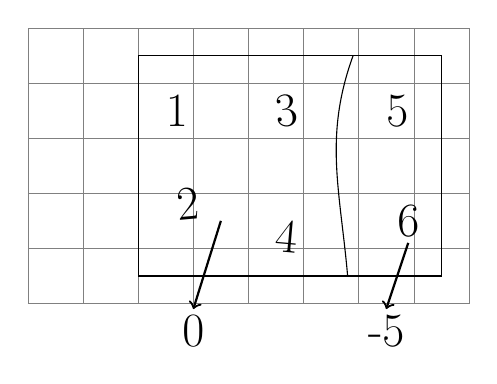
\begin{tikzpicture}[scale=0.7]
		\draw[help lines] (0,0) grid (8,5);
		% Box mit Omega
		\draw (2,0.5) -- (2,4.5) -- (7.5,4.5) -- (7.5,0.5) -- (2,0.5);
		% Zahlen in der Box
		\foreach \x/\y/\n/\r in {2.7/3.5/1/0,2.9/1.8/2/5,4.7/3.5/3/7,4.7/1.2/4/-5,6.7/3.5/5/0,6.9/1.5/6/0}
		\node[rotate=\r] at (\x,\y) {\LARGE \n};
		% Schrägstrich in der Box 
		\draw (5.8,0.5) to [out=95,in=250] (5.9,4.5);
		% Pfeile an den Unterteilung : 0
			%definiere (lokale Variabeln)
			\def \x {3} 
			\def \y {-0.1}
		\draw[thick,->] (\x+0.5,1.5) -- (\x,\y);
		\node at (\x,\y-0.4) {\LARGE 0};
		% Pfeile an den Unterteilung : 1
			%definiere (lokale Variabeln)
			\def \x {6.5} 
			\def \y {-0.1}
		\draw[thick,->] (\x+0.4,1.1) -- (\x,\y);
		\node at (\x,\y-0.4) {\LARGE -5};
	\end{tikzpicture}
\end{minipage}
%
\begin{minipage}{0.55\linewidth}
	\underline{Gewinnspiel:}
		\begin{itemize}
			\item bei $5,6 \to$ Verlust von $5EURO$
			\item bei $1,2,3$ oder $4$ Gewinn in Höhe der doppelten Augenzahl 
		\end{itemize}
\end{minipage}

	ZV $Z =$ Gewinn / Verlust in EURO mit 
	Realisationsmöglichkeiten: $-5,2,4,6,8$\\

\begin{minipage}{0.45\linewidth}
\begin{tikz}[scale=0.5]
	\draw[help lines] (0,0) grid (8,5);	
\end{tikz}
\end{minipage}
\begin{minipage}{0.55\linewidth}
	\underline{Wahrscheinlichkeitsverteilung von $Z$}
	\begin{tabular}{c | c c c c c}
		$Z_i$ 	&  -5		& 	2		&		4		& 	6		&		8		\\
		\hline
		\vspace{1em} $ P( Z = z_1)$ & $\frac{2}{6}$ & $\frac{1}{6}$ & $\frac{1}{6}$ & $\frac{1}{6}$ & $\frac{1}{6}$ 
	\end{tabular}
\end{minipage}

\begin{minipage}{0.45\linewidth}
\begin{tikz}[scale=0.5]
	\draw[help lines] (0,0) grid (8,5);	
\end{tikz}
\end{minipage}
\begin{minipage}{0.55\linewidth}
	\underline{Verteilungsfunktion von $Z$}: $F(z) = P(Z \leq z), z\in \R$
	\begin{tabular}{c | c c c c c}
		$Z_i$ 	&  -5		& 	2		&		4		& 	6		&		8		\\
		\hline
		\vspace{1em} $ P( Z \leq z_1)$ & $\frac{2}{6}$ & $\frac{3}{6}$ & $\frac{4}{6}$ & $\frac{5}{6}$ & $\frac{6}{6}=1$ 
	\end{tabular}
\end{minipage}
~\\
$\begin{aligned}
	E(Z)	&= z_1 \cdot \underbrace{P(Z=z_1)}_{p_1} + z_2 \cdot \underbrace{P(Z=z_2)}_{p_2}
						+ \cdot + z_5 \cdot \underbrace{P(Z=z_5)}_{p_5}\\
				&= z_1 p_1 + z_2 p_2 + \dots + z_5 p_5\\
				&= -5 \cdot \frac{2}{6} + 2 \cdot \frac{1}{6} + 4 \cdot \frac{1}{6}
				+ 6 \cdot \frac{1}{6}	+ 8\cdot \frac{1}{6}\\
				&= + \underline{\underline{1,\ov{6}}}
\end{aligned}$
\begin{tabbing}
	\underline{Interpretation:} \= Spielen wir dieses Spiel sehr oft, wird der 
		Gewinn im Durchschnitt bei $1,67$EURO liegen.
\end{tabbing}
\end{bsp}

\underline{deskriptiv}: Varianz und Standardabweichung \\
Varianz \dots mittlere quadrierte Abweichung von arithmetischen Mittel
	$$ \sum (\alpha_i - \ov{x})^2 h_i = s_x^2$$
$\alpha_i$ $\leftrightarrow$ Realisationsmöglichkeiten $x_i$ \\
$\ov{x}$ $\leftrightarrow$ $E(X)$	\\
$h_i$ $\leftrightarrow$ $p_i$

\underline{Varianz einer ZV $X$}: 
	$Var(X) = \sigma^2 = \sum_{i=1}^{k}(x_i - E(X))^2 p_i		
		= E((X-E(X))^2)$, wobei $p_i = P(X=x_i)$\\
Erwartungswert der quadrierten Differenzen für viele Versuchswiederholungen gilt  

\begin{tabular}{p{0.5\linewidth} p{0.5\linewidth}}
\hfill 23 & 23 \hfill\\
\end{tabular}

%%%%%%%%%%%%%%%%%%%%%%%%%%%%%%%%%%%%%%%%%%%%%%%%%%%%%%%%%
\def\varA{\mbox{
	\begin{tabular}{@{}l@{}}
		berechnet mit Realisations-\\möglichkeiten und $p_i$
	\end{tabular}
	}
	\hspace{0em}
}
\def\varB{\mbox{
	\begin{tabular}{@{}l@{}}
		berechnet mit Realisationen bzw.\\ Beobachtungen und $h_i$
	\end{tabular}
	}
	\hspace{0em}
}
%%%%%%%%%%%%%%%%%%%%%%%%%%%%%%%%%%%%%%%%%%%%%%%%%%%%%%%%%

	$$ \underbrace{Var(X)}_{\varA} \approx \; \underbrace{s_x^2}_{\varB}$$

%\begin{tabular}{p{0.15\linewidth} | p{0.1\linewidth} | p{0.1\linewidth} | p{0.1\linewidth} | p{0.1\linewidth} | p{0.1\linewidth}}
\begin{tabular}{c | c | c | c | c | c l }
$z_i$	  & -5 & 2 & 4 & 6 & 8\\
\hline   
$p_i$  &  $\frac{2}{6}$  & $\frac{1}{6}$ & $\frac{1}{6}$ & $\frac{1}{6}$ & $\frac{1}{6}$ \\
$(z_i -1,\ov{6})^2$ & 44,44 & 0,11 & 5,44 & 18,78 & 40,11 \\
$(z_i -1,\ov{6})^2$ & 14,81 & 0,018 & 0,91 & 3,13 & 6,685 \\
\end{tabular}
\begin{tabular}{l}
\\ \\ \\
$\Sigma = \underline{\underline{25,55}}$	
\end{tabular}

$Var(Z) = \sigma_Z^2 = 25,55$\\
Standardabweichung: $\sigma_Z = \sqrt{Var(Z)} = \sqrt{25,55} = $ \underline{\underline{5,05}} \\

Im Mittel weichen die Realisationen von $Z$ (also der Gewinn) um 5,05 EURO von durchschnittlichen bzw. erwarteten Gewinn 1,67 EURO ab.\\

ZV $Y$ sei auch ein Gewinn in einem Glückspiel

\begin{tabular}{c | c c c c}
	$y_i$		&		0		&		1		&		5		&		10	\\
	\hline
	$p_i$		&	0,35	& 0,5		&		0,1	&	0,05  \\
	$(y_i -\underbrace{E(Y)}_{= 1,5})^2$
					&	2,25	&	0,25	&	12,15	&	72,25
\end{tabular}

$\begin{aligned}
	E(Y) &= 0,35 \cdot 0 + 0,5 \cdot 1 + 0,1 \cdot 5 + 0,05 \cdot 10 =
	\underline{\underline{1,5}} EURO \\
%
	E(Z) &= +1,67  EURO \\
%
	Var(Y) &= 2,25 \cdot 0,35 + 0,25 \cdot 0,5 + 12,25 \cdot 0,1 +
	72,26 \cdot 0,05 \\
	&= \text{\underline{\underline{5,75}}} = \sigma_y^2\\
%
	\sigma_y &= \sqrt{5,75} = \underline{\underline{2,4}} \\
%
	\sigma_z &= \underline{\underline{5,05}} \\
\end{aligned}$

$$\begin{aligned}
	E(Y)		 &<	E(Z) \\
	\sigma_Y &< \sigma_Z
\end{aligned}$$

Summe von zwei Würfeln $ = X$

$\begin{aligned}
\Omega = \{& \overbrace{(1,1)}^{X=2}, \overbrace{(1,2)}^{X=3}, \dots , 
	\overbrace{(1,6)}^{X=7} \\
					 & \underbrace{(2,1)}_{X=3}, \underbrace{(2,2)}_{X=4}, 
	\underbrace{(2,6)}_{X=8} \\
	 				 & \underbrace{(6,1)}_{X=7}, \underbrace{(6,2)}_{X=8}, \dots ,
	\underbrace{(6,6)}_{X=12}\} \quad \text{mögliche Ergebnisse}
\end{aligned}$
\par
alle Ergebnisse haben die gleiche W. \\
6x6 mögliche Ergebnisse = Anzahl der möglichen Ergebnisse

$\begin{aligned}
\text{z.B.} \quad & P(X = 3) = P(\set{(1,2), (2,1)}) = \frac{2}{36}\\
						& P(X = 7) = \frac{6}{36} = \frac{1}{6}
\end{aligned}$

$(1,6) , (6,1)$\\
$(2,5), (5,2) $\\
$(3,4), (4,3)$ \\

\begin{tabular}{c | c | c}
$x_i$	&	$p_i$	&	$P(X \le x_i)$ \\
\hline
	2		&	1/36	&			1/36			\\
	3		&	2/36	&			3/36			\\	
	4		&	3/36	&			6/36			\\	
	5		&	4/36	&		 10/36			\\	
	6		&	5/36	&		 15/36			\\	
	7		&	6/36	&		 21/36			\\	
	8		&	5/36	&		 26/36			\\	
	9		&	4/36	&		 30/36			\\	
	10	&	3/36	&		 33/36			\\	
	11	&	2/36	&		 35/36			\\	
	12	&	1/36	&		  1/36			\\	
\end{tabular}
%
$\begin{aligned}
	P(X \leq 7) &= \frac{21}{36} \\
	P(X \geq 7) &= P(X > 6) = 1 - P(\leq 6) =  21/36 \\
	P(X < 7) &= P(X \leq 6) = \frac{15}{36} \\
	P(X > 7) &= 1 - P(X \leq 7) = \frac{15}{36} \\
	\\
	P(5 < X \leq 10) &= 
\end{aligned}$
